\documentclass[12pt,letterpaper]{article}
\usepackage{preamble}
\usepackage[brazil]{babel}
\usepackage[utf8]{inputenc}
\usepackage{enumitem}
\usepackage{comment}

%%%%%%%%%%%%%%%%%%%%%%%%%%%%%%%%%%%%%%%%%%
%%%% Edit These for yourself
%%%%%%%%%%%%%%%%%%%%%%%%%%%%%%%%%%%%%%%%%%
\newcommand\course{IA753}
\newcommand\hwnumber{2}
\newcommand\userID{Heitor S. Fernandes - RA: 074096}

\begin{document}
\centerline{\textbf{\Large Trabalho Computacional \hwnumber}}

\centerline{\text{ Linguagem utilizada: Python }}

\section*{Tarefa 1}
\begin{enumerate}[label=(\alph*)]  %,leftmargin=!,labelindent=5pt]
    \item Para selecionar devidamente os neurônios, primeiro o arquivo é carregado e em seguida os diferentes vetores são separados: tempo, spikes e força. Então, são detectados os índices únicos de neurônios e selecionados apenas aqueles com índice menor que 100. É feita mais uma seleção para ficar apenas os neurônios com pelo menos 50 {\it spikes} e, então, é feito o sorteio de 10 neurônios.
    
    %O sinal foi carregado a partir do arquivo \emph{signal.txt}. A frequência de amostragem ${f_s = 500 Hz}$ foi utilizada para calcular o tamanho do passo temporal: ${dt = 1/f_s = 0.002}$ segundos . A partir de ${dt}$ e do número de amostras ${N = 1000}$, foi criado um vetor tempo, indo de 0.000 a 19.998 segundos. O sinal no tempo pode ser visto na figura \ref{fig:1}, abaixo.
%\begin{comment}
    \begin{lstlisting}[language=Python][basicstyle=\small]
from scipy.io import loadmat
import numpy as np; np.set_printoptions(precision=3)
import matplotlib.pyplot as plt; plt.ion()
# Carregar o arquivo
data = loadmat('../data/tc2ex1.mat')

spikes_all = data['spikes']
force = data['force']
force.shape = (max(force.shape),)
t = data['time']
t.shape = (max(t.shape),)

# Selecionar os indices menores que 100
neurons_id_all = np.array(np.unique(spikes_all[:,1]),dtype=int)
neurons_id_100 = neurons_id_all[neurons_id_all<100]

# Selecionar apenas os neuronios com pelo menos 50 spikes
good_neurons_id = np.array([i for i in neurons_id_100 if len(spikes_all[spikes_all[:,1]==i])>50])

# Sortear 10 neuronios
N = 10
#np.random.seed(1)
neurons_id = np.random.choice(good_neurons_id,N,replace=False)
spikes = np.array([spk for spk in spikes_all if int(spk[1]) in neurons_id])
num_spikes = np.array([len(spikes[spikes[:,1]==i]) for i in neurons_id])
print(u'Neurônios sorteados:')
print([n for n in neurons_id])
print(u'Número de spikes:')
print([n for n in num_spikes])
    \end{lstlisting}
%\end{comment}

\newpage
    Se usarmos a linha \lstinline{np.random.seed(1)} para reproduzir a condição aleatória, teremos os seguintes neurônios e números de {\it spikes}.
    
    Neurônios sorteados:
    [93, 84, 32, 28, 79, 18, 99, 82, 69, 63]

    Número de spikes:
    [106, 87, 116, 113, 134, 126, 93, 120, 84, 102]

    \item
    As variabilidades da força e dos ISIs foram calculadas a partir do instante ${1000ms}$, descartando o transitório. Abaixo, os valores encontrados para cada métrica.
    
    {\it i)} Força média no registro: ${73.62 N}$
    
    {\it ii)} Desvio padrão da força no registro: ${5.66 N}$
    
    Coef. de variação da força no registro: ${7.69 \%}$
      
    {\it iii)} Dados sobre os ISIs:
    
        \begin{table}[H]
        \centering
        \begin{tabular}{llllll}
            Neurônio & ISI médio [ms] & ISI ${\sigma}$ [ms] & ISI CV [\%] & Coef. Assim. & Curtose \\ 
            93 & 94.08 & 18.84 & 20.03 & 1.18 & 1.58 \\
            84 & 114.29 & 31.04 & 27.16 & 1.04 & 0.86 \\
            32 & 87.02 & 13.10 & 15.05 & 0.48 & -0.43 \\
            28 & 87.85 & 13.05 & 14.85 & 1.36 & 4.28 \\
            79 & 73.75 & 8.48 & 11.50 & 0.34 & -0.14 \\
            18 & 78.88 & 11.17 & 14.16 & 0.70 & 0.36 \\
            99 & 105.81 & 25.57 & 24.17 & 1.63 & 3.94 \\
            82 & 82.96 & 14.61 & 17.61 & 1.39 & 4.51 \\
            69 & 118.59 & 31.80 & 26.82 & 1.60 & 3.57 \\
            63 & 98.70 & 23.13 & 23.44 & 1.24 & 2.47 \\
        \end{tabular}
        \end{table}
    
    Abaixo, os histogramas dos dez neurônios selecionados. Observa-se que todos os neurônios possuem estatísticas de disparo com coeficiente positivo, gerando assimetria para a esquerda, o que pode ser visto na figura. Os disparos dos neurônios 32 e 79 levam a uma distribuição platicúrtica (curtose menor que zero, seguindo a definição de Fisher, como a função utilizada \lstinline{scipy.stats.kurt}), enquanto que os neurônios 28, 69, 82 e 99 apresentaram distribuição dos ISIs muito leptocúrtica, indicando uma maior dispersão quando comparado a uma distribuição normal, além de, também, apresentarem os maiores coeficientes de assimetria.
    
        \begin{figure}[H]
            \centering
            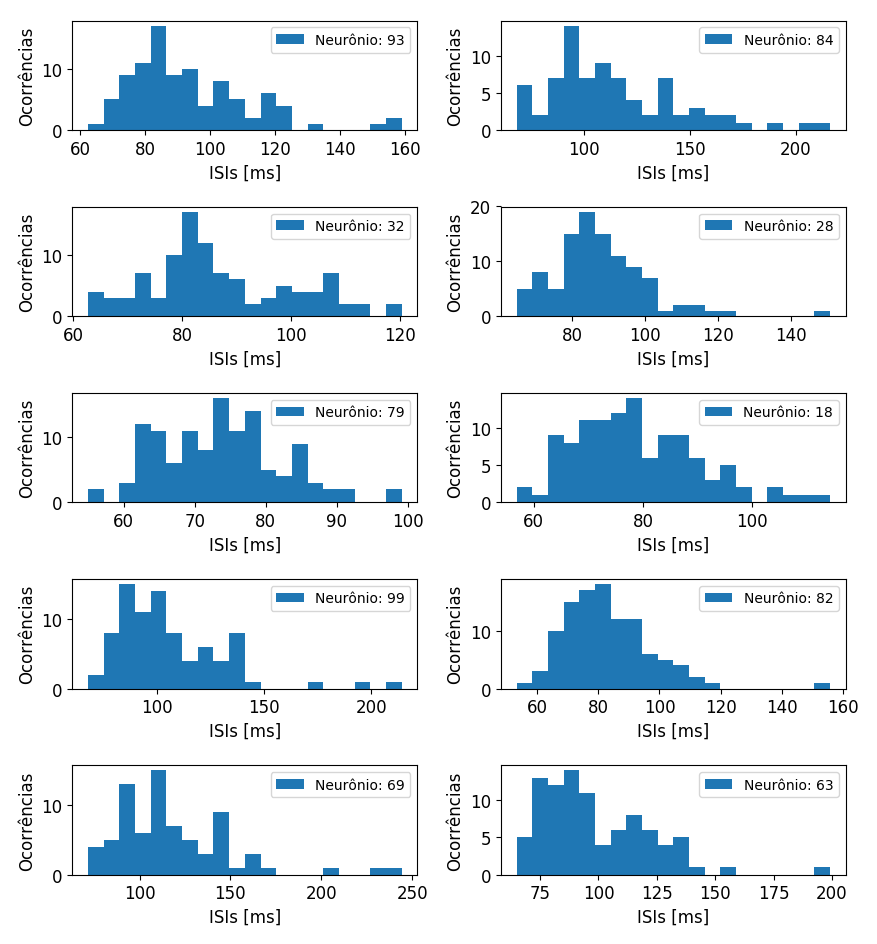
\includegraphics[width=15cm]{TC2/images/histogramas.png}
            \caption{Histogramas dos ISIs dos neurônios selecionados.}
            \label{fig:1}
        \end{figure}
    
    
%    Foi utilizado o comando \lstinline{np.fft.rfft} para obter a FFT do sinal (figura \ref{fig:2}). Outra maneira seria utilizar a FFT complexa (\lstinline{np.fft.fft}) e utilizar a apenas a parte real da resposta. O comando \lstinline{np.fft.rfftfreq} fornece as frequências de amostragem, porém em unidade adimensional. Para calibrar o eixo das abscissas em Hertz foi calculada a resolução espectral como o inverso do tempo se amostragem, isto é, ${df = {1/(dt*N)} = 0.05 Hz}$, e utilizado o número de amostras $N$.
    
   % $${f_{Hz} = f_{adim}*df*N = {f_{adim} \over {dt*N}} *N = {f_{adim} \over dt}}$$
    
    \item
    Para estimar as frequências instantâneas de disparo dos neurônios foram criados os vetores de impulsos de mesmo tamanho que o vetor {\it tempo}, com o valor $1/T_s$ (período de amostragem $T_s = 0.05ms$) nos instantes definidos pelos {\it spikes} (Figura \ref{fig:impulsos}). Então, foi criada a janela {\it Hanning} de $500/T_s = 10000$ amostras com área unitária (Figura \ref{fig:hann}), significando ${500 ms}$:
    
       \begin{lstlisting}[language=Python][basicstyle=\small]
window = np.hanning(500/dt)
window = window/np.trapz(window)
    \end{lstlisting}
        
        \begin{figure}[H]
            \centering
            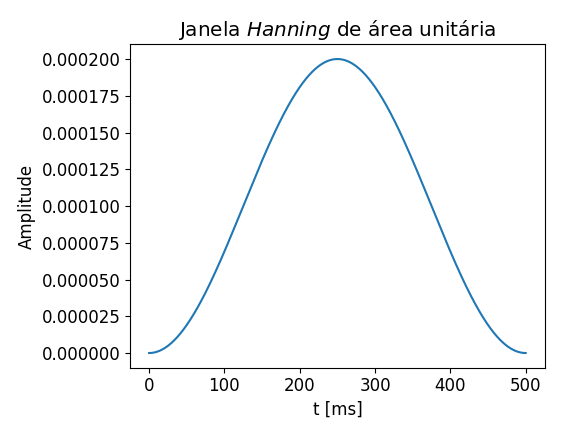
\includegraphics[width=10cm]{TC2/images/hann.png}
            \caption{Janela do tipo {\it Hanning} de área unitária, duração de ${500 ms}$ com período de amostragem de ${0.05 ms}$.}
            \label{fig:hann}
        \end{figure}
    
        \begin{figure}[H]
            \centering
            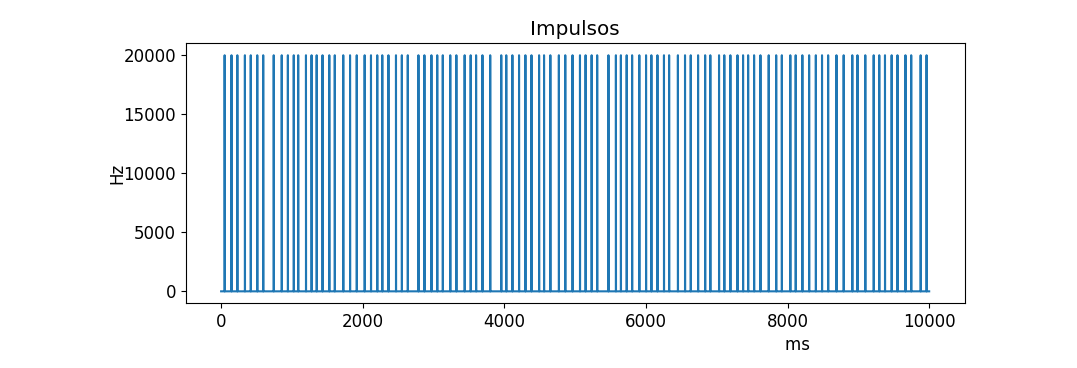
\includegraphics[width=15cm]{TC2/images/impulsos.png}
            \caption{Impulsos referentes aos disparos do neurônio 93.}
            \label{fig:impulsos}
        \end{figure}
    
    As frequências instantâneas estimadas estão representadas na Figura \ref{fig:ifreqs}.
    
        \begin{figure}[H]
            \centering
            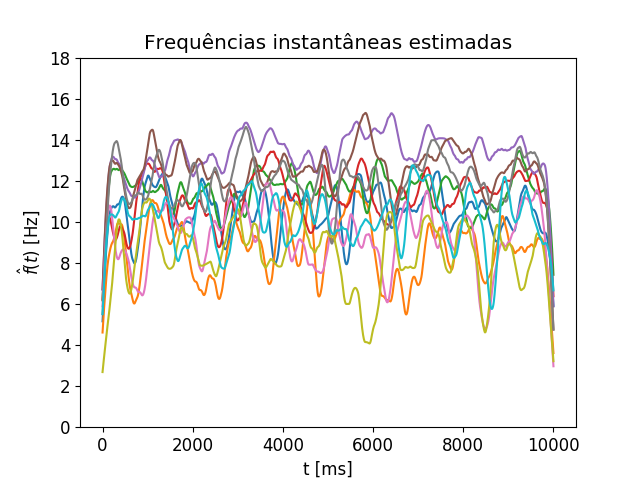
\includegraphics[width=13cm]{TC2/images/inst_freqs.png}
            \caption{Frequências instantâneas estimadas por janelamento do tipo {\it Hanning}.}
            \label{fig:ifreqs}
        \end{figure}
    
    \item
    Foi considerado como estacionário o intervalo entre ${800ms}$ e ${9500ms}$, no qual não há mais efeito transitório.
    
    {\it i)} Correlação cruzada entre a força e as frequências estimadas.
    
    Para calcular a correlação cruzada foi utilizada a função \lstinline{scipy.signal.correlate} dividida pelo número de amostras dos vetores, porém, apenas após subtrair o valor médio de cada vetor e após passá-lo pela função \lstinline{scipy.signal.detrend} para remover tendências lineares. As funções correlação cruzada entre a força e as frequências estimadas podem ser vistas na Figura \ref{fig:xcforcafreq}.
    
    As funções de correlação cruzada entre a força e as frequências de dispato estimadas apresendam, quase todas, pico perto do atraso zero, indicando alta correlação entre estas grandezas, o que faz sentido quando considerado que, em indivíduos saudáveis e em condições normais, os disparos dos neurônios motores dão origem a potenciais de ação nas fibras musculares e, subsequentemente, a geração de força. O fato do pico não estar exatamente em lag zero, indica que há uma tendência fortíssima de haver um atraso entre os dois mecanismos (disparo de neurônio e geração de força), podendo representar o tempo entre o disparo dos neurônio e o acoplamento excitação-contração das fibras musculares até a geração efetiva de força.
        
        \begin{figure}[H]
            \centering
            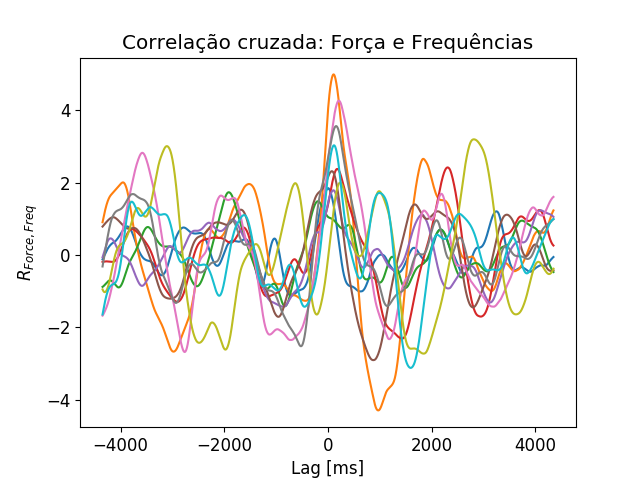
\includegraphics[width=15cm]{TC2/images/corr_force-freqs.png}
            \caption{Correlação cruzada: força e frequências estimadas.}
            \label{fig:xcforcafreq}
        \end{figure}
    
    {\it ii)} Correlação cruzada entre pares de frequências estimadas.
    
    As funções correlação cruzada entre os pares de frequência estimada foram calculadas de maneira similar. Para os pares de frequências estimadas também foi desenhada e destacada em linha mais espessa, na Figura \ref{fig:cxfreqfreq}, a média de todas as correlações cruzadas entre os pares, a fim de observar um efeito global de correlação entre as frequências de disparo.
    
    O pico perto do atraso zero observado na média das funções de correlação entre os pares de frequência indica a alta correlação entre os disparos dos neurônios e que a modulação das frequências de disparo são praticamente simultâneas (pico perto de zero). Isto corrobora para o conceito de {\it common drive} apresentado por De luca e Erim \cite{DeLuca1994}.
        
        \begin{figure}[H]
            \centering
            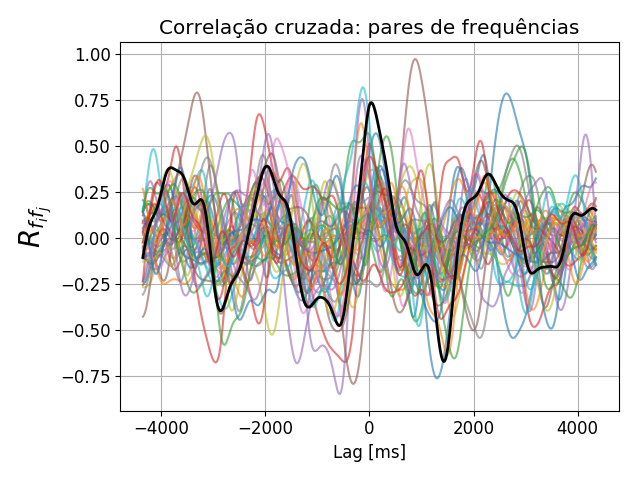
\includegraphics[width=15cm]{TC2/images/corr-freq-freq.png}
            \caption{Correlação cruzada: pares de frequências estimadas e média.}
            \label{fig:cxfreqfreq}
        \end{figure}
    
    
\end{enumerate}

\section*{Tarefa 2}

\begin{enumerate}[label=(\alph*)]  %,leftmargin=!,labelindent=5pt]
    \item Conforme visto em aula, sabemos que a correlação cruzada entre a entrada e a saída de um sistema LIT (linear invariante no tempo), ${R_{xy}}$, pode ser escrita como:

    
    $$
    R_{xy}(t) = h(t) * R_{xx}(t)
    $$
    
    Onde ${h(t)}$ é a resposta do sistema a uma entrada ${y(t)}$ e ${R_{xx}(t)}$ é a função de autocorrelação da entrada $x(t)$.
    Aplicando a transformada de Fourier nos dois termos da equação acima, teremos:
    
    $$
    \mathcal{F} \{R_{xy}(t)\} = \mathcal{F} \{h(t)\} \mathcal{F} \{R_{xx}(t)\}
    $$
    
    Utilizando o teorema de Wiener-Kintchine, como visto em aula, teremos:
    
    $$
    S_{XY}(jw) = \mathcal{F} \{R_{xy}(t)\}
    $$
    $$
    \Rightarrow
    S_{XY}(jw) = H(jw) * S_{XX}(jw)
    $$
    $$
    \Rightarrow H(jw) = {S_{XY}(jw) \over S_{XX}(jw)}
    $$

    \item
    Para estimar a resposta em frequência, primeiro foram calculados o espectro cruzado entre a entrada e a saída $S_{XY}(jw)$ e o autoespectro da entrada $S_{XY}(jw)$ utilizando a função \lstinline{scipy.signal.csd}, entrando com a frequência de amostragem $fs = 1000 Hz$ e obtendo o espectro desejado e as frequências amostradas.
    
    Em seguida, foi calculado $H(jw)$ e plotados os diagramas de Bode em magnitude e fase, vistos na Figura \ref{fig:bodeb}. Foi necessário utilizar a função \lstinline{numpy.unwrap} para corrigir um salto na fase que a função \lstinline{numpy.angle} causa por gerar apenas valores entre $-\pi$ e $\pi$.
            
        \begin{figure}[H]
            \centering
            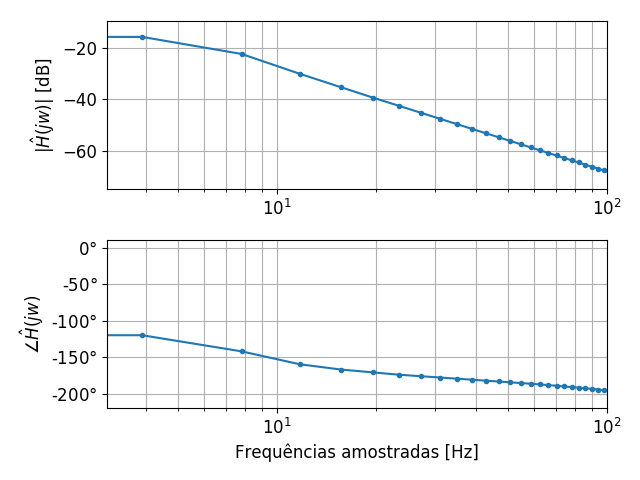
\includegraphics[width=15cm]{TC2/images/bode_itemb.png}
            \caption{Diagramas de Bode da resposta em frequência estimada $\hat{H}(jw)$.}
            \label{fig:bodeb}
        \end{figure}
    
    \item
    Para encontrar $\omega_n$, foi feita a substituição de $s$ por $j\omega$ e, então, de $\omega$ por $\omega_n$.
    
    $$
    H(s) = {{\omega_n}^2 \over {s^2 + 2\omega s + {\omega_n}^2}     }  (1)
    $$
    $$
    H(j\omega) = {{\omega_n}^2 \over {(j\omega_n)^2 + 2{\omeg_na}^2  + {\omega_n}^2}     }
    $$
    $$
    H(j\omega) = {{\omega_n}^2 \over {-\omega_n^2 + 2{\omeg_na}^2  + {\omega_n}^2}     }
    $$
    $$
    H(j\omega) = {{\omega_n}^2 \over {2j{\omega_n}^2} } = {1 \over 2j}
    $$
    
    Indicando uma fase de $-90 graus$. Procurando um deslocamento de fase de -90 graus no diagramad de fase da Figura \ref{fig:bodeb}, obtermos, aproximadamente, $\omega_n = 2Hz$.
    
    Substituindo o valor encontrado na Equação (1), $\omega_n = 2Hz$, e gerando um $H(j \omega)$, temos novos diagramas de bode, vistos com comparação com o estimado, na Figura \ref{fig:bodec}.
    
            \begin{figure}[H]
            \centering
            \includegraphics[width=15cm]{TC2/images/bode_c.png}
            \caption{Diagramas de Bode da resposta em frequência estimada $\hat{H}(jw)$.}
            \label{fig:bodec}
        \end{figure}

    
\end{enumerate}



\bibliographystyle{IEEEtran}
\bibliography{library}
\end{document}
